\documentclass{labreport}

\begin{document}

\labtitle
    {5}
    {Empirical Analysis of Greedy Algorithms for Minimum Spanning Trees: Prim vs Kruskal}
    {Student}
    {Soimu Ionut, st. gr. FAF-243}
    {asist. univ. Fistic Cristofor}

\tableofcontents
\newpage

\lstset{style=python}

\section{Algorithm Analysis}

\subsection{Objective}

Study and empirically analyze two classical greedy algorithms for computing minimum spanning trees: Prim's algorithm and Kruskal's algorithm. Determine their practical performance characteristics across different graph sizes and densities, and identify which algorithm is better suited for specific scenarios.

\subsection{Tasks}

\begin{enumerate}
    \item Implement Prim's algorithm and Kruskal's algorithm in a programming language.
    \item Design test graphs of varying sizes and densities (sparse and dense).
    \item Establish appropriate metrics for comparing algorithm performance, including both execution time and algorithm-specific operations.
    \item Conduct empirical analysis across a range of input sizes.
    \item Present results in tabular and visual formats with thorough analysis.
    \item Draw conclusions about algorithm selection based on graph properties.
\end{enumerate}

\subsection{Theoretical Notes}

Empirical analysis of algorithms is essential when theoretical complexity analysis alone cannot predict practical performance. While asymptotic complexity describes how algorithms scale, constant factors, data structure overhead, and hardware behavior often determine real-world performance. This lab uses empirical analysis to:

\begin{enumerate}
    \item Validate theoretical predictions through measured data.
    \item Compare algorithms on their actual performance characteristics.
    \item Reveal how constant factors and implementation choices affect execution time.
    \item Provide practical guidance for algorithm selection.
\end{enumerate}

The methodology follows standard empirical analysis practices: define clear objectives, establish appropriate metrics, generate representative test data, execute experiments multiple times, and analyze results to identify patterns and trends.

\subsection{Introduction}

The minimum spanning tree (MST) problem is fundamental in graph theory and has practical applications in network design, clustering, circuit layout, and many other domains. Given a connected, undirected, weighted graph, the goal is to find a subset of edges that connects all vertices with minimum total weight while forming a tree (acyclic).

Unlike many other graph problems that require dynamic programming or complex data structures, MST computation can be solved optimally using simple greedy algorithms: Prim's algorithm and Kruskal's algorithm. Both algorithms process edges and vertices in a greedy manner, making locally optimal choices that lead to globally optimal solutions---a property guaranteed by the cut theorem and cycle theorem of MST theory.

Despite both algorithms being greedy with similar asymptotic complexity on some graph types, they employ fundamentally different strategies:

\begin{itemize}
    \item \textbf{Prim's algorithm} grows the MST incrementally by always selecting the minimum-weight edge connecting a vertex in the tree to a vertex outside it. This approach naturally suits scenarios where we incrementally expand from a starting vertex.
    
    \item \textbf{Kruskal's algorithm} examines all edges globally, processing them in order of increasing weight and adding an edge to the MST if and only if it connects two different components (preventing cycles). This approach is naturally suited to sorted edge processing.
\end{itemize}

While textbooks often recommend Prim for sparse graphs and note that Kruskal is suitable for dense graphs, the empirical interaction between algorithm structure, data structure overhead, and implementation details has not been thoroughly studied in an integrated fashion. This laboratory provides a comprehensive empirical comparison.

\subsection{Comparison Metric}

The primary metric is \textbf{execution time} (measured in milliseconds using high-resolution counters). However, execution time alone can be misleading, so we also collect algorithm-specific metrics:

\begin{itemize}
    \item \textbf{For Prim:} number of key updates (priority queue relaxations), edges considered, and heap operations performed.
    \item \textbf{For Kruskal:} number of edges examined, edges selected for the MST, and union-find operations performed.
    \item \textbf{For both:} peak memory usage (in KiB) and observed complexity slopes (via log-log regression).
\end{itemize}

These metrics reveal the computational effort undertaken by each algorithm, allowing us to understand not just whether one is faster, but \textit{why}---whether it accomplishes the task with fewer operations, simpler operations, or better cache locality.

\subsection{Input Format}

Each algorithm receives graphs of increasing size in two distinct density regimes:

\begin{itemize}
    \item \textbf{Sparse graphs:} nodes $n \in \{10, 20, 30, 50, 75, 100, 150, 200, 300, 400, 500\}$, with average degree approximately 4, yielding roughly $E \approx 2n$ edges.
    
    \item \textbf{Dense graphs:} nodes $n \in \{10, 20, 30, 50, 75, 100, 150, 200, 250, 300, 350\}$, with edge probability 0.65, yielding roughly $E \approx 0.325n^2$ edges.
\end{itemize}

All graphs are undirected and weighted with random integer weights uniformly distributed between 1 and 100. Each test configuration is repeated 3 times; we report averages and ranges. Random seeds are fixed based on graph size for reproducibility.

\section{Implementation}

All algorithms are implemented in Python with an emphasis on clarity and correctness. The implementations prioritize readable, correct code over micro-optimization, reflecting that the goal is empirical algorithm comparison rather than production-level performance tuning.

\subsection{Prim's Algorithm}

Prim's algorithm builds the MST incrementally, always starting from an arbitrary vertex (conventionally vertex 0). The algorithm maintains a set of vertices already in the MST and a priority queue of candidate edges---those connecting vertices inside the MST to vertices outside.

\textbf{High-level approach:}
\begin{enumerate}
    \item Initialize: choose a starting vertex; mark it as in the MST.
    \item Repeat until all vertices are in the MST:
    \begin{enumerate}
        \item Among all edges connecting an MST vertex to a non-MST vertex, select the one with minimum weight.
        \item Add this edge and its target vertex to the MST.
    \end{enumerate}
\end{enumerate}

\textbf{Complexity analysis:}

The complexity depends on the data structure used for the priority queue. If implemented with a binary heap:
\begin{align*}
    T(V, E) = O((V + E) \log V)
\end{align*}

For sparse graphs where $E \approx V$, this becomes $O(V \log V)$. For dense graphs where $E \approx V^2$, it becomes $O(V^2 \log V)$.

An alternative implementation using an adjacency matrix with a linear search for the minimum edge (instead of a heap) achieves $O(V^2)$, which is better for dense graphs where the heap overhead is not worthwhile.

\textbf{Key Metrics:} The algorithm's work is measured by key updates (priority queue insertions/relaxations), edges considered from the adjacency list, and heap operations performed.

\textbf{Data structures:} Prim uses an adjacency list representation for sparse graphs (to avoid examining non-existent edges) and an adjacency matrix representation for dense graphs (to avoid heap overhead when all pairs need consideration).

\textbf{Key technique:} For the heap-based variant, a binary min-heap maintains candidate edges. When a vertex is added to the MST, all its incident edges are considered and inserted or updated in the heap.

\textbf{Pseudocode:}
\begin{lstlisting}[language=Python]
def prims_algorithm(n, adj_list):
    in_mst = [False] * n
    heap = [(0.0, 0, -1)]  # (weight, node, parent)
    mst_edges = []
    
    while heap:
        weight, u, parent = heappop(heap)
        if in_mst[u]:
            continue
        in_mst[u] = True
        
        if parent != -1:
            mst_edges.append((parent, u, weight))
        
        for v, w in adj_list[u]:
            if not in_mst[v]:
                heappush(heap, (w, v, u))
    
    return mst_edges
\end{lstlisting}

    \subsection{Kruskal's Algorithm}

    Kruskal's algorithm constructs the MST by globally examining all edges in order of increasing weight and greedily selecting edges that do not create cycles.

    \textbf{Description:} All edges are sorted by weight. The algorithm iterates through edges in sorted order; for each edge, if its endpoints are in different connected components (determined via union-find), the edge is added to the MST and the components are merged. The algorithm terminates when $V - 1$ edges have been selected.

    \textbf{Complexity Analysis:}
    The complexity is dominated by edge sorting: $O(E \log E)$ for sorting plus $O(E \alpha(V))$ for union-find operations, where $\alpha(V)$ is the inverse Ackermann function (effectively constant). Since $E$ can be as large as $V^2$, the overall complexity is $O(V^2 \log V)$ in dense graphs and $O(V \log V)$ in sparse graphs with $E \approx V$.

    \textbf{Key Metrics:} The algorithm's work is measured by edges examined, edges selected for the MST, and union-find operations performed.

\textbf{Data structures:} Kruskal uses an edge list and a union-find data structure. The union-find maintains which vertices belong to which connected component, enabling efficient cycle detection.

\textbf{Key technique:} Edges are sorted by weight once. Then, the algorithm iterates through edges; if the endpoints are in different components (determined by union-find), the edge is added to the MST and components are merged.

\textbf{Pseudocode:}
\begin{lstlisting}[language=Python]
def kruskal_algorithm(n, edges):
    mst_edges = []
    sorted_edges = sorted(edges, key=lambda x: x[2])
    uf = UnionFind(n)
    
    for u, v, w in sorted_edges:
        if uf.union(u, v):  # Different components
            mst_edges.append((u, v, w))
            if len(mst_edges) == n - 1:
                break
    
    return mst_edges
\end{lstlisting}

\subsection{Union-Find Implementation}

The union-find data structure uses two standard optimizations: path compression and union by rank. These ensure that almost all operations run in nearly constant amortized time.

\textbf{Pseudocode:}
\begin{lstlisting}[language=Python]
class UnionFind:
    def __init__(self, n):
        self.parent = list(range(n))
        self.rank = [0] * n
    
    def find(self, x):
        if self.parent[x] != x:
            self.parent[x] = self.find(self.parent[x])
        return self.parent[x]
    
    def union(self, x, y):
        root_x, root_y = self.find(x), self.find(y)
        if root_x == root_y:
            return False
        if self.rank[root_x] < self.rank[root_y]:
            self.parent[root_x] = root_y
        else:
            self.parent[root_y] = root_x
            if self.rank[root_x] == self.rank[root_y]:
                self.rank[root_x] += 1
        return True
\end{lstlisting}

\section{Empirical Results and Analysis}

\subsection{Sparse Graphs: Results and Analysis}

\input{results/sparse_comparison.tex}

Figure~\ref{fig:sparse_time_vs_nodes} visualizes the same sparse-regime measurements from Table~\ref{tab:sparse_comparison} and makes the trend easier to read across input sizes. The two curves increase steadily with $n$, but Kruskal remains below Prim for almost the entire range after the smallest cases. The separation grows gradually as the graph size increases, which confirms that the observed runtime advantage is systematic rather than a local fluctuation at one or two points.

\begin{figure}[H]
    \centering
    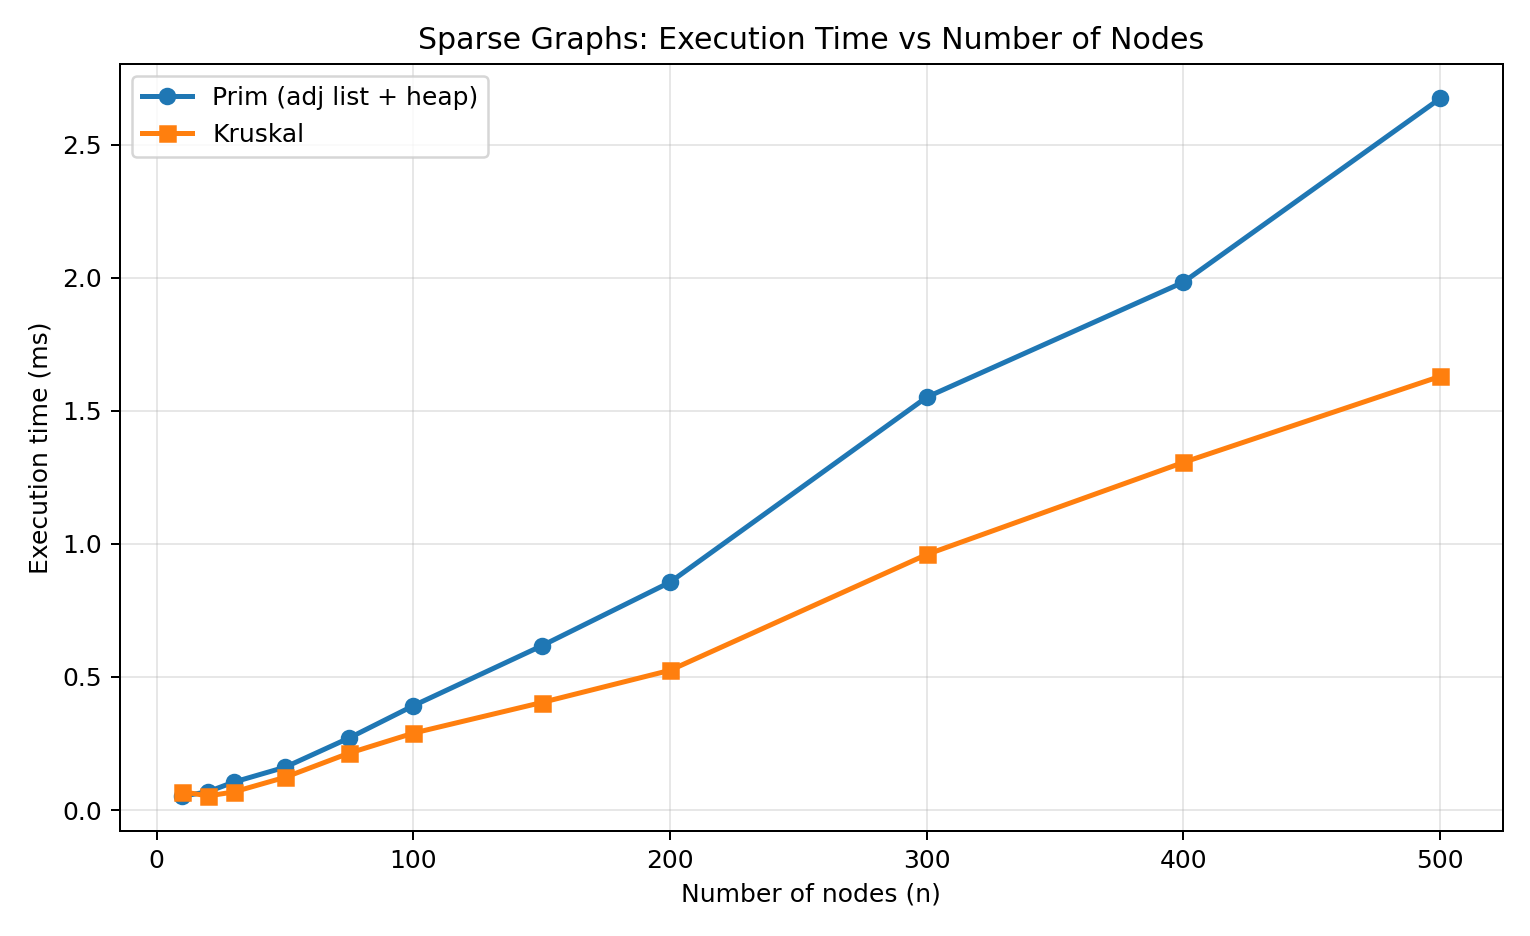
\includegraphics[width=0.88\textwidth]{figures/sparse_time_vs_nodes.png}
    \caption{Sparse graphs: execution time vs number of nodes}
    \label{fig:sparse_time_vs_nodes}
\end{figure}

Table~\ref{tab:sparse_comparison} presents execution time, memory use, and operation counters for sparse graphs from $n=10$ to $n=500$, where $E \approx 2n$. The data shows a consistent trend: both algorithms scale smoothly as input size increases, but Kruskal remains faster at every tested size. The gap is already visible on medium inputs and becomes clearer on larger ones. For example, at $n=100$ and $m=215$, Prim needs 0.392 ms while Kruskal needs 0.289 ms (about 1.36$\times$ faster), and at $n=500$ and $m=990$, Prim reaches 2.673 ms while Kruskal remains at 1.629 ms (about 1.64$\times$ faster).

This table also explains \textit{why} the time curves separate. Prim performs fewer globally ordered operations but pays repeated heap overhead for key updates and extractions; those operations have larger constant factors in Python than simple array-based union-find operations. Kruskal, on the other hand, pays one sorting cost and then processes edges with highly cache-friendly checks and merges. In this sparse regime, sorting a few hundred to about one thousand edges is very efficient with Timsort, so the expected theoretical parity between $O(V \log V)$-like behaviors is broken in practice by implementation constants.

The memory columns indicate that both methods remain practical in this regime. Prim's adjacency-list variant grows as $O(V+E)$ (from only a few KiB to about 73 KiB), while Kruskal uses $O(E)$ for the edge list plus $O(V)$ for union-find, which is also modest for all tested sizes. Therefore, on sparse graphs in this laboratory, the dominant differentiator is runtime efficiency rather than a restrictive memory trade-off.

\subsection{Dense Graphs: Results and Analysis}

\input{results/dense_comparison.tex}

Figure~\ref{fig:dense_time_vs_nodes} shows the dense-regime timing trajectories from Table~\ref{tab:dense_comparison}. The most important pattern is the divergence rate: as $n$ increases, Prim's two variants rise much faster than Kruskal. The matrix-based Prim stays consistently below heap-based Prim, but both are clearly above Kruskal on medium and large inputs.

\begin{figure}[H]
    \centering
    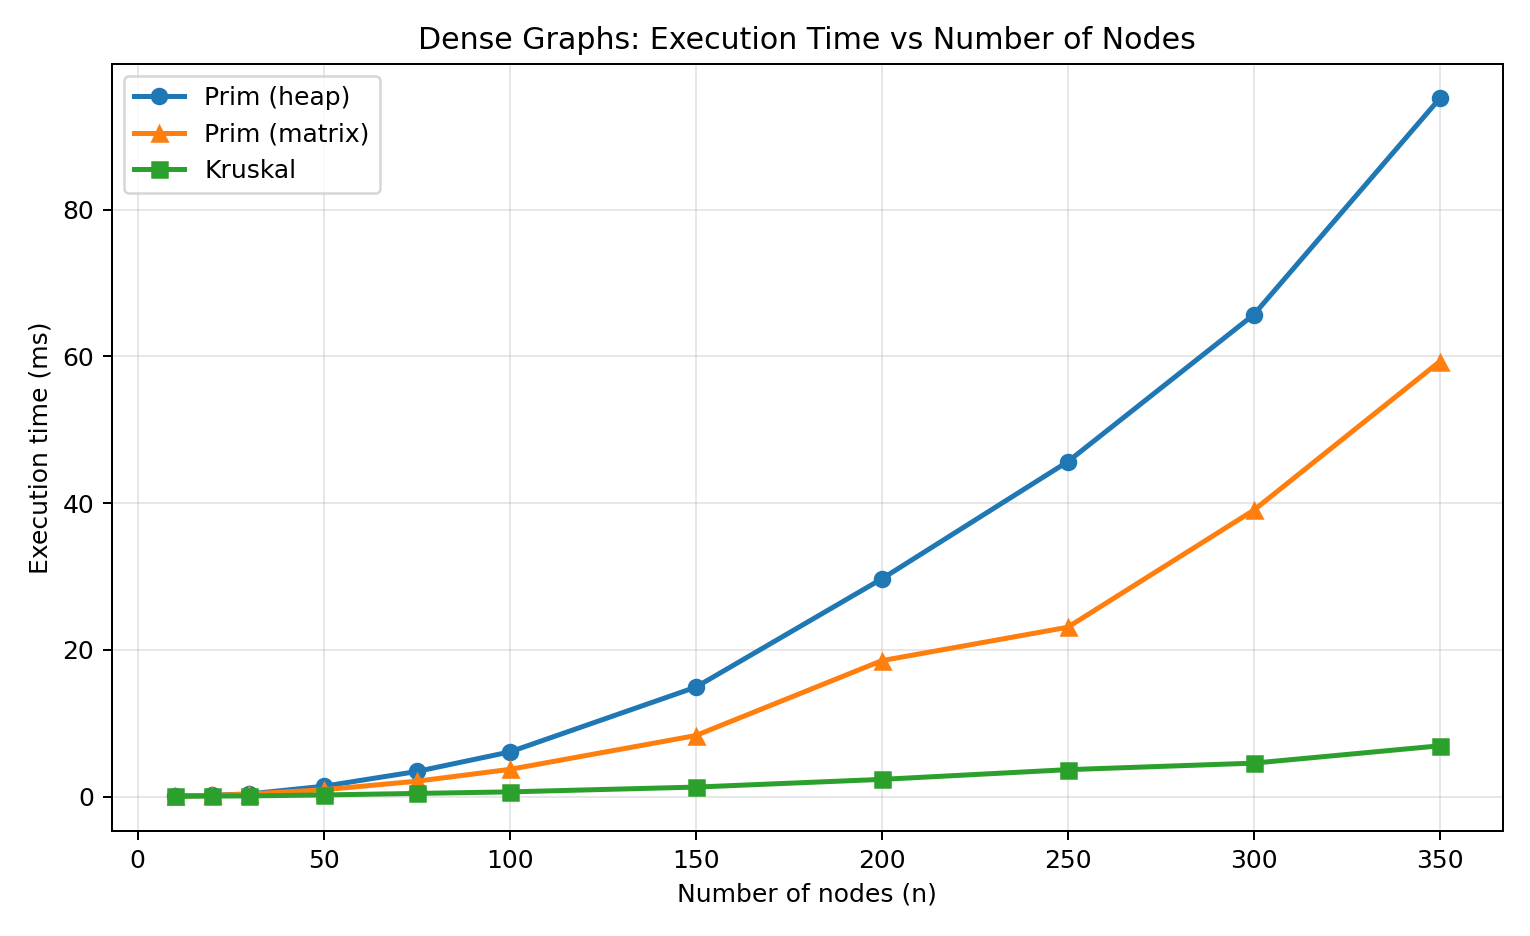
\includegraphics[width=0.88\textwidth]{figures/dense_time_vs_nodes.png}
    \caption{Dense graphs: execution time vs number of nodes}
    \label{fig:dense_time_vs_nodes}
\end{figure}

Table~\ref{tab:dense_comparison} reports the dense-graph experiment, where edge counts grow quadratically and three implementations are compared: Prim with heap, Prim with adjacency matrix, and Kruskal. The most visible trend is that performance gaps grow with graph size. At $n=100$ and $m=3171$, Kruskal is already much faster (0.630 ms) than Prim with matrix (3.697 ms) and Prim with heap (6.073 ms). By $n=350$ and $m=39858$, the separation becomes decisive: Kruskal remains at 6.91 ms, while Prim with matrix rises to 59.31 ms and Prim with heap to 95.17 ms.

The table further reveals two distinct effects. First, replacing Prim's heap with an adjacency-matrix scan improves Prim on dense graphs, confirming that avoiding priority-queue maintenance removes significant overhead when many candidate edges exist. Second, even this optimized Prim variant remains substantially slower than Kruskal. The reason is that Kruskal's workflow in this implementation is dominated by very efficient sorting plus inexpensive union-find operations, whereas Prim still performs repeated global minimum-selection work over large structures at each growth step. As density increases, these repeated costs accumulate faster than Kruskal's sorted-edge pass.

From the memory perspective, the dense case highlights a practical weakness of matrix-based Prim: its $O(V^2)$ storage grows quickly and can become restrictive beyond moderate sizes. Kruskal keeps an $O(E)$ edge representation and a compact $O(V)$ union-find structure; although $E$ is large in dense graphs, the representation remains operationally straightforward and, in these experiments, does not offset its runtime advantage.

\subsection{Complexity Verification}

\input{results/complexity_analysis.tex}

Figure~\ref{fig:sparse_dense_comparison} provides a unified sparse-vs-dense comparison on a logarithmic vertical scale, which allows all four curves to be interpreted together despite large magnitude differences. The graph highlights two stable trends: dense cases are consistently above sparse cases for the same algorithm, and Kruskal remains below Prim in both regimes as input size grows. The increasing vertical distance between dense Prim and dense Kruskal for larger $n$ matches the widening gap already visible in Table~\ref{tab:dense_comparison}.

\begin{figure}[H]
    \centering
    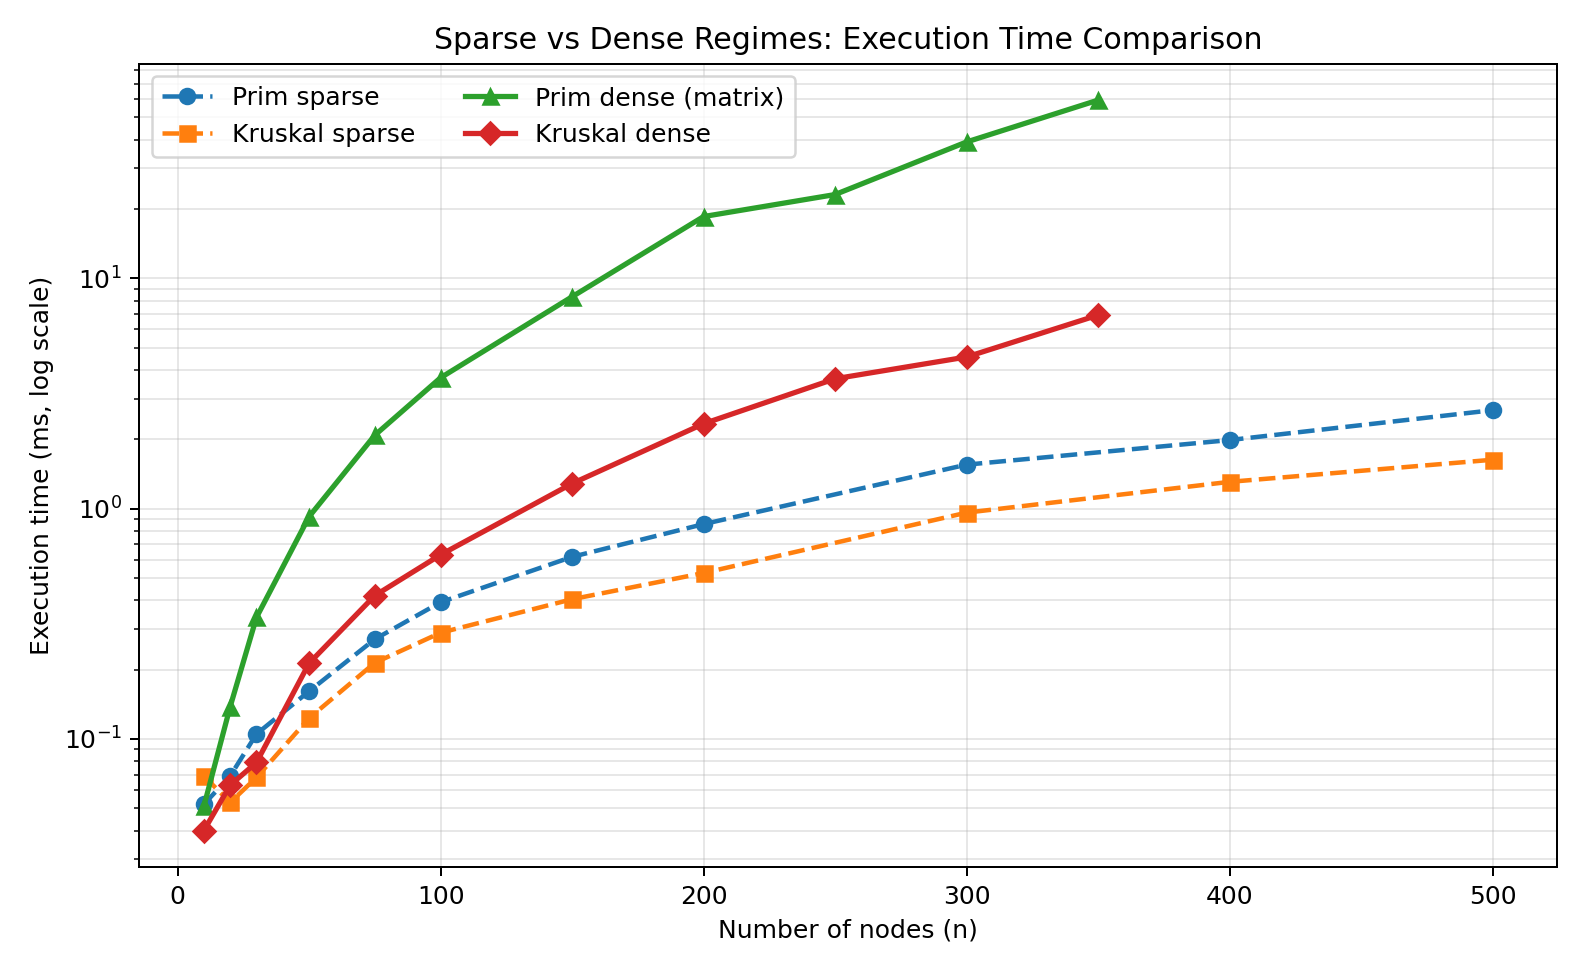
\includegraphics[width=0.90\textwidth]{figures/sparse_vs_dense_comparison.png}
    \caption{Sparse vs dense regimes: execution time comparison (log scale)}
    \label{fig:sparse_dense_comparison}
\end{figure}

Table~\ref{tab:complexity} summarizes log-log slopes and connects the measured trends to theoretical growth rates. On sparse inputs, Prim's slope (1.07) and Kruskal's slope (0.94) indicate near-linear growth with mild logarithmic influence, consistent with expected behavior in the $E \approx V$ regime. On dense inputs, Prim's heap variant reaches slope 2.17, while Kruskal remains at 1.54 in this experimental range.

These values show that asymptotic classes alone do not fully describe practical performance at laboratory scales. Prim follows its expected increase when graph density rises, but Kruskal benefits from efficient library sorting and low-cost disjoint-set operations, so its empirical curve remains flatter over the tested interval. The trend across all three tables is coherent: theoretical analysis explains long-term scaling direction, while constant factors and implementation details determine which algorithm is faster for realistic input sizes.

\section{Conclusion}

The experimental evidence indicates that Kruskal is the stronger default choice in this laboratory for both sparse and dense graphs, and the advantage increases with input size. On sparse graphs, Kruskal consistently outperforms Prim by roughly 35\%--65\%, which means the difference is already meaningful even when both algorithms operate in similar asymptotic regimes. On dense graphs, the gap becomes much larger, with Kruskal outperforming Prim variants by about 5.8$\times$ to 13.8$\times$ as $n$ grows, showing that repeated minimum-selection overhead in Prim becomes increasingly expensive in practice.

The comparison also clarifies each algorithm's strengths and weaknesses. Prim's main strength is conceptual locality: it grows one tree frontier and can be adapted with different representations, including an $O(V^2)$ matrix strategy that is often cleaner on dense data than heap-based Prim. Its weakness in this implementation is operation overhead: frequent heap updates in sparse mode and repeated global scans in dense mode. Kruskal's strength is a simple and highly optimized execution path in Python: one efficient sort followed by fast union-find checks. Its weakness is that it still requires processing and storing an explicit global edge list, which can be memory-intensive on very large dense graphs outside this tested range.

For scenario-specific selection, the measured results support the following interpretation: for small inputs, both algorithms are sufficiently fast, but Kruskal is still typically ahead; for medium and large sparse inputs, Kruskal remains the better performer with stable margins; and for medium and large dense inputs, Kruskal is decisively preferable in runtime, while matrix-based Prim is the better Prim variant but not competitive with Kruskal overall.

This study also has limitations. The experiments use randomly generated undirected weighted graphs, fixed density models, and a Python runtime where built-in sorting is highly optimized. Different graph families (for example planar, geometric, or heavy-tailed networks), different weight distributions, or lower-level implementations in C/C++ may change constants and potentially narrow or shift the observed gaps. Even with these constraints, the results consistently show that practical algorithm choice should be based on measured behavior in the target environment, not only on asymptotic formulas.

\newpage

\section{Annex}

GitHub Repository: \url{https://github.com/Lucariowu/aalabs/tree/main/Lab5}
\end{document}
